\section{Introduction}

% What is the problem?
Migrating resources is a useful tool for optimizing performance for systems
that service highly accessed data\footnote{In this paper, we use the term
``data" to refer to the partitioned key-value pairs AND file system metadata.}
but deciding how to make the migrations is a risky trade-off. Data can be
distributed to alleviate overloaded servers or it can be concentrated to
exploit locality. These techniques are at odds and selecting the wrong technique
can have catastrophic consequences. For example, migrating data to an
already overloaded server or increasing the network hops by spreading data
across an underutilized cluster will impact performance negatively.

% Why is concentration vs. distribution difficult?
Unfortunately, deciding which optimization to use is difficult to reason about,
especially with the scale and complexity of today's HPC architectures. While
the mechanisms are usually built into the systems, the policies often times
less refined and much more sensitive to the workload. So a system may have the
ability exploit locality using techniques like bulk operations, multiple
partition strategies, secondary indexes, and caching but deciding when, where,
and how to use them is workload dependent and difficult to figure out.

% What we did in the paper
This paper takes an API designed to migrate file system metadata and applies it
to an HPC key-value store.  The API helps control distribution and
concentration by letting the administrator define how to migrate load, where to
migrate load, and how much load to migrate. While designed for a different
domains, this API encompasses many of the same properties we need for an HPC
key-value store, namely:

\begin{itemize}
  \item services small/frequent requests
  \item popularity drives distribution
  \item locality drives concentration
\end{itemize}

\begin{figure}[t]
  \noindent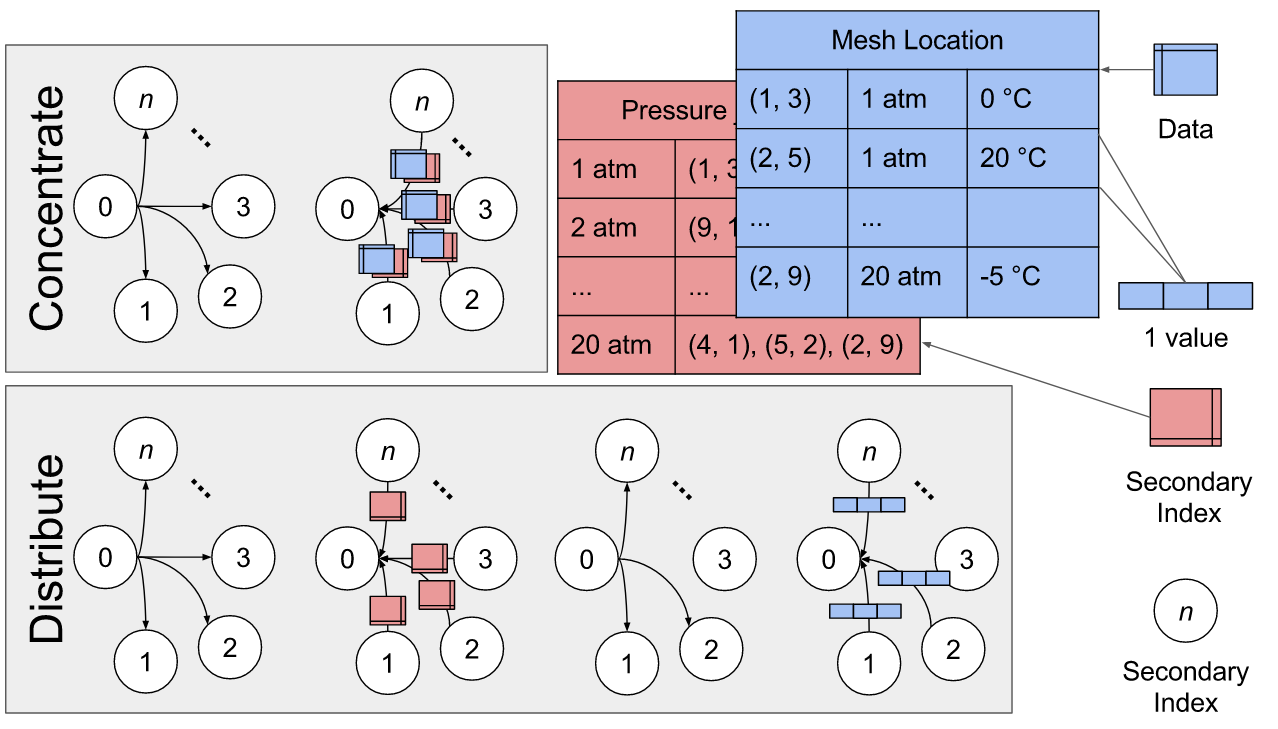
\includegraphics[width=19pc,angle=0]{figures/example.png}\\
  \caption{For a multi-part query with locality, migrating for distribution
  (solution 1) takes more RPCs while migrating for concentration (solution 2)
  risks of overloading the client.}
  \label{fig:example}
\end{figure}

% Why is HXHIM a good fit?
To show the efficacy of this approach, we examine multi-part queries that have
both a high computational footprint, which suggests distribution to avoid hot
spots, and data locality, which alternatively encourages concentration so the
system can use its functionality for secondary indices, bulk operations, and
key redistribution.  The motivating example for this integration is finding the
maximum value \(x\) of the neighbors in a mesh of another maximum value \(y\).
For example, finding the highest temperatures of the neighbors of mesh cells
with the highest pressure. Given that the hash is defined by mesh location,
finding the highest pressure is one RPC per server.  Unfortunately, even
with an index based on the maximum pressures, finding the highest temperatures
for {\it neighboring} cells with the highest pressures requires an additional
RPC per server. 

% What can the API do?
Specifically, the API helps us explore the space of solutions for these types
of queries. As shown in Figure~\ref{fig:example}, queries with locality have
two solutions: (1) pull the index and re-query every server, or (2) pull the
index and partial set of results that can be satisfied locally. Solution 1
emphasizes distribution and incurrs extra RPCs while Solution 2 opts to
concentrate data at the expense of data transfer, consistency issues, and
increased memory usage.  Both options have advantages but inserting an API to
control the mechanisms helps future programmers quickly evaluate both options
and design solutions for their workload.

% What do we contribute?
In this paper, we make the following contributions:

\begin{enumerate}

  \item protype that controls concentration and distribution using the bulk
  operations, secondary indicies, and cursor types mechanisms
  from~\cite{greenberg:hotstorage2015-mdhim}. 

  \item quantifies benefits of server/client-side caching, many small messages,
  and bulk operations.

\end{enumerate}
